\item {\bf Implicit Regularization}

Recall that in the overparameterized regime (where the number of parameters is larger than the number of samples), typically there are infinitely many solutions that can fit the training dataset perfectly, and many of them cannot generalize well (that is, they have large validation errors). However, in many cases, the particular optimizer we use (e.g., GD, SGD with particular learning rates, batch sizes, noise, etc.) tends to find solutions that generalize well. This phenomenon is called implicit regularization effect (also known as algorithmic regularization or implicit bias). 

In this problem, we will look at the implicit regularization effect on two toy examples in the overparameterized regime: linear regression and a quadratically parameterized model. For linear regression, we will show that gradient descent with zero initialization will always find the minimum norm solution (instead of an arbitrary solution that fits the training data), and in practice, the minimum norm solution tends to generalize well. For a quadratically parameterized model, we will show that initialization and batch size also affect generalization.

\begin{enumerate}
    \input{04-implicitreg/01-linear-overfitting}
    
    \input{04-implicitreg/02-linear-overfitting}
    
    \item \points{4c} \textbf{Minimum norm solution generalizes well}

For this sub-question, we still work with the setup of parts (a) and (b). We use the following datasets:
\begin{center}
	\texttt{src-implicitreg/ir1\_train.csv, ir1\_valid.csv}
\end{center}
Each file contains $d+1$ columns. The first $d$ columns in the $i$-th row represents $x^{(i)}$, and the last column represents $y^{(i)}.$ In this sub-question, we use $d=200$ and $n=40$.

Using the formula in sub-question (b), \textbf{compute} the minimum norm solution using the training dataset. Then, \textbf{generate} three other different solutions with zero costs and different norms using the formula in sub-question (a).
The starter code is in \texttt{src-implicitreg/submission.py} and you should implement the \texttt{get\_minimum\_norm\_solution} and \texttt{get\_different\_n\_solutions} functions.  
Your generated plot should demonstrate that the minimum norm solution generalizes well and should be similar to the following plot:

\begin{figure}[H]
	\centering
	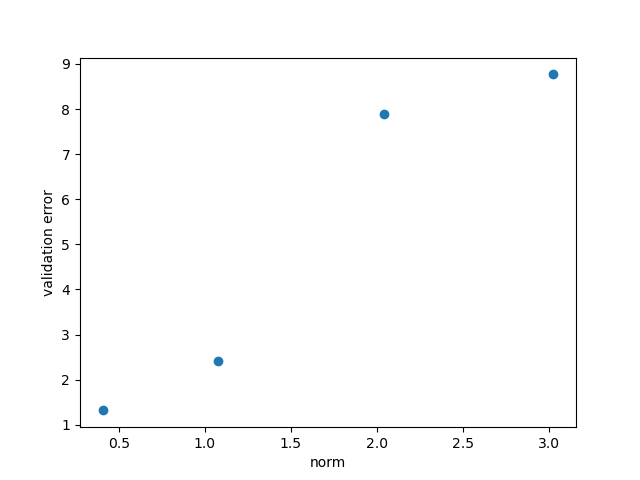
\includegraphics[width=.5\linewidth]{04-implicitreg/implicitreg_linear.png}
	\caption{Visual impaired students can access the corresponding desmos plot \href{https://www.desmos.com/calculator/b5ef1cvybm}{here}}
\end{figure}
	
	\input{04-implicitreg/04-linear-gd}

	\input{04-implicitreg/05-qp-overfitting}

	\item \points{4f} \textbf{Implicit regularization of initialization}

We still work with the setup in part (e).
For this sub-question, we use the following datasets:
\begin{center}
	\texttt{src-implicitreg/ir2\_train.csv, ir2\_valid.csv}
\end{center}
Each file contains $d+1$ columns. The first $d$ columns in the $i$-th row represents $x^{(i)}$, and the last column represents $y^{(i)}.$ In this sub-question, we use $d=200$ and $n=40$.

First of all, the gradient of the loss has the following form:
\begin{align}
	\nabla_\theta J(\theta,\phi)&=\frac{1}{n}\sum_{i=1}^{n}((x^{(i)})^\top (\theta^{\odot 2} -\phi^{\odot 2})-y^{(i)})(\theta\odot x^{(i)}),\\
	\nabla_\phi J(\theta,\phi)&=-\frac{1}{n}\sum_{i=1}^{n}((x^{(i)})^\top (\theta^{\odot 2} -\phi^{\odot 2})-y^{(i)})(\phi\odot x^{(i)}).
\end{align}
You don't need to prove these two equations. They can be verified directly using the chain rule.

Using the formula above, run gradient descent with initialization $\theta=\alpha \mathbf{1}, \phi=\alpha\mathbf{1}$ with $\alpha\in \{0.1, 0.03, 0.01\}$ (where $\mathbf{1}=[1,1,\cdots,1]\in\R^{d}$ is the all-1's vector) and learning rate $0.08$. We provide the starter code in \texttt{src-implicitreg/submission.py} and you should implement the \texttt{QP.gradient} and \texttt{QP.train\_GD} functions. Your generated plot should be looking like the following:

\begin{figure}[H]
	\centering
	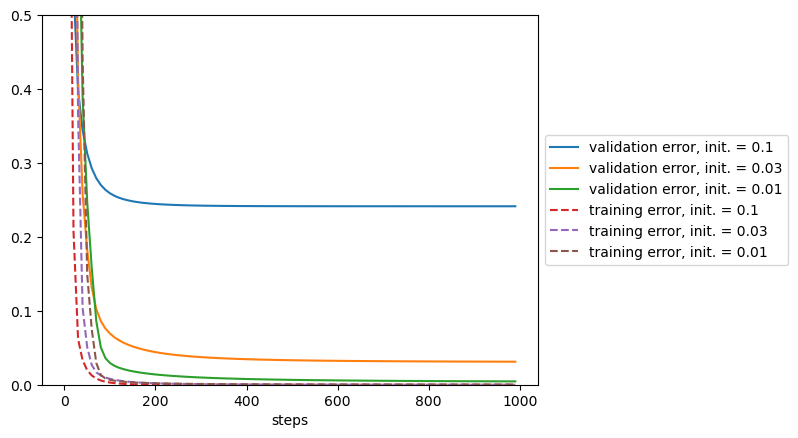
\includegraphics[width=.7\linewidth]{04-implicitreg/implicitreg_quadratic_initialization.png}
	\caption{Visual impaired students can access the corresponding desmos plot \href{https://www.desmos.com/calculator/scqmmrwkuj}{here}}
\end{figure}

\textit{Remark:} Your plot is expected to demonstrate that the initialization plays an important role in the generalization performance---different initialization can lead to different global minimizers with different generalization performance. In other words, the initialization has an implicit regularization effect. 

	\input{04-implicitreg/07-qp-initialization}

	\item \points{4h} \textbf{Implicit regularization of batch size}

We still work with the setup in part (e). For this sub-question, we use the same dataset and starter code as in sub-question (f). We will show that the noise in the training process also induces implicit regularization. In particular, the noise introduced by \emph{stochastic} gradient descent in this case helps generalization. \textbf{Implement} the SGD algorithm in the \texttt{QP.train\_SGD} function and run it with batch size $\{1, 5, 40\}$, learning rate $0.08$, and initialization $\alpha=0.1$. For simplicity, the code for selecting a batch of examples is already provided in the starter code.

Your generated plot should like like the following:

\begin{figure}[H]
    \centering
    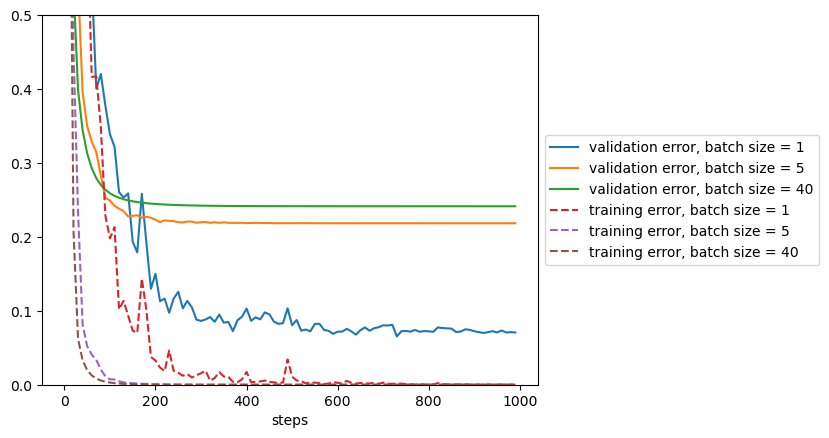
\includegraphics[width=.7\linewidth]{04-implicitreg/implicitreg_quadratic_batchsize.png}
    \caption{Visual impaired students can access the corresponding desmos plot \href{https://www.desmos.com/calculator/0gdthqojwa}{here}}
\end{figure}

The plot shows that the stochasticity in the training process is also an important factor in the generalization performance --- in our setting, SGD finds a solution that generalizes better. In fact, a conjecture is that stochasticity in the optimization process (such as the noise introduced by a small batch size) helps the optimizer to find a solution that generalizes better. This conjecture can be proved in some simplified cases, such as the quadratically parameterized model in this sub-question (adapted from the paper \href{https://arxiv.org/abs/2006.08680}{HaoChen et al., 2020}), and can be observed empirically in many other cases.

\textbf{Files to Submit: }\texttt{src-implicitreg/submission.py}

	\input{04-implicitreg/09-qp-batchsize}
\end{enumerate}
